\documentclass[12pt, letterpaper]{article}

% --- Packages ---
\usepackage[utf8]{inputenc}
\usepackage{geometry}
\geometry{margin=1in}
\usepackage{setspace}
\usepackage{enumitem}
\usepackage{titlesec}
\usepackage{fancyhdr}
\usepackage{lineno}
\usepackage{amsmath}
\usepackage{tikz}
\usetikzlibrary{shapes.geometric, arrows.meta, positioning, fit, calc}

% --- Header & Footer ---
\pagestyle{fancy}
\fancyhf{}
\rhead{\small PROVISIONAL PATENT APPLICATION}
\lhead{\small \today}
\cfoot{\thepage}
\setlength{\headheight}{15pt}
\addtolength{\topmargin}{-3pt}

% --- Section Formatting ---
\titleformat{\section}{\large\bfseries\uppercase}{\thesection.}{1em}{}
\titleformat{\subsection}{\normalsize\bfseries}{\thesubsection.}{1em}{}

% --- Line Spacing & Numbering ---
\doublespacing
\linenumbers

\begin{document}

\begin{center}
    {\Large \textbf{SYSTEM AND METHOD FOR PREEMPTIVE CYBERSECURITY THREAT CONTAINMENT REDIRECTION AND Hardware-Enforced Architectural Reconfiguration USING NEURO-SYMBOLIC AI AND CONTINUOUS-TIME GRAPH ORDINARY DIFFERENTIAL EQUATIONS}}
\end{center}

\vspace{1em}

\section*{Abstract of the Disclosure}
A computer-implemented system and method for preemptive cybersecurity architectural reconfiguration and polymorphic threat containment redirection. The system utilizes a multi-modal Neuro-Symbolic Artificial Intelligence layer to ingest disparate unstructured data, including text, binary structures, and architectural diagrams, generating permutation-invariant Threat Conditioning Vectors via a Causal Threat Directed Acyclic Graph (DAG). A Temporal Asset Graph (TAG) is continuously mapped via local operating system metrics and extended Berkeley Packet Filter (eBPF) probes. A Counterfactual Temporal Graph Neural Network (C-TGNN) leveraging Continuous-Time Graph Ordinary Differential Equations (CT-GODE) simulates infinite-hop lateral movement pathways. In response to a time-decaying Blast Radius Score (BRS) exceeding a threshold, a remediation controller dynamically synthesizes and executes polymorphic eBPF routing logic within software processes to perform Semantic Traffic Shaping, thereby transforming susceptible nodes into ephemeral kernel-level containment nodes prior to active exploitation.

\section{Background of the Invention}
\subsection{Field of the Invention}
The present disclosure relates generally to advanced cybersecurity defense mechanisms, and more particularly, to computing systems, software-based orchestration, and algorithmic methods for predicting, prioritizing, and automatically mitigating zero-day threats and Advanced Persistent Threat (APT) campaigns using Continuous-Time Graph Ordinary Differential Equations, Neuro-Symbolic AI, and dynamic software containment redirection.

\subsection{Description of Related Art}
Modern organizations face highly sophisticated, multi-stage cyberattacks. Defensive operations typically rely on Security Information and Event Management (SIEM) systems and Security Orchestration, Automation, and Response (SOAR) tools. These legacy systems predominantly operate on reactive paradigms and static heuristic matching against outdated Configuration Management Databases (CMDBs).

Furthermore, conventional SOAR platforms are structurally bound to deterministic, boolean logic (e.g., "If IP = Malicious, Block Port"). These reactive playbooks are fundamentally incapable of responding to probabilistic, non-deterministic threat forecasting. SOAR platforms rely on centralized, binary enforcement mechanisms (e.g., firewall API calls) that induce high latency and are easily bypassed by sophisticated adversaries who morph their TTPs faster than central playbooks can update. There exists a critical need for decentralized, probabilistic enforcement that operates pre-emptively on counterfactual threat simulations rather than deterministic intelligence triggers, integrating directly at the micro-architectural and operating system kernel levels to physically sever and deceive threat vectors.

\section{Summary of the Invention}
The following presents a simplified summary of one or more embodiments in order to provide a basic understanding of such embodiments. This summary is not an extensive overview of all contemplated embodiments, and is intended to neither identify key or critical elements of all embodiments nor delineate the scope of any or all embodiments.

In one aspect of the present disclosure, a system for preemptive, dynamic architectural reconfiguration is provided. The system comprises a Neuro-Symbolic AI abstraction layer fusing a custom transformer topology (incorporating Cross-Attention and a Graph Isomorphism Network) with deterministic First-Order Logic validation via Z3. The system ingests multi-modal data, including text, binary code snippets, hexadecimal memory dumps, and image-based architectural diagrams, transforming them into a permutation-invariant Threat Conditioning Vector.

In parallel, telemetry leverages eXpress Data Path (XDP) offloading to DPUs and SmartNICs, fusing eBPF network telemetry with deep micro-architectural telemetry from CPU Performance Monitor Units (PMUs). This constructs a nanosecond-precision Temporal Asset Graph (TAG).

A Counterfactual Continuous-Time Graph Neural Network (C-TGNN) processes this telemetry, substituting discrete time steps with Continuous-Time Graph Ordinary Differential Equations (CT-GODE), specifically utilizing a pure PyTorch Runge-Kutta 4th Order (RK4) solver, to model asynchronous, multi-hop propagation. A zero-trust out-of-band remediation controller synthesizes polymorphic, P4-language routing logic and state-aware eBPF payloads, executed directly on network interface controllers (NICs) or within operating system kernel space, establishing an immutable micro-perimeter that performs deceptive Semantic Traffic Shaping, functioning as an ephemeral containment node without deploying additional virtual machines.

\section{Brief Description of the Drawings}
\begin{itemize}
    \item \textbf{FIG. 1} is a schematic block diagram illustrating the overall system architecture, in accordance with an embodiment of the present invention.
    \item \textbf{FIG. 2} is a flowchart illustrating an exemplary method for multi-modal ingestion, predictive simulation, and Static Packet Reflection.
    \item \textbf{FIG. 3} is a detailed block diagram illustrating the Neuro-Symbolic Multi-Modal Ingestion Pipeline and Causal Threat DAG generation.
    \item \textbf{FIG. 4} is a schematic diagram depicting the construction of the nanosecond-precision Temporal Asset Graph (TAG) via eBPF and PMU telemetry.
    \item \textbf{FIG. 5} is a functional diagram of the Counterfactual Continuous-Time Graph Neural Network (C-TGNN) executing the CT-GODE algorithm.
    \item \textbf{FIG. 6} illustrates the Static eBPF Packet Reflector Controller injecting semantic shaping rules into operating system kernel space and NIC ASICs.
\end{itemize}

\begin{figure}[htbp]
\centering
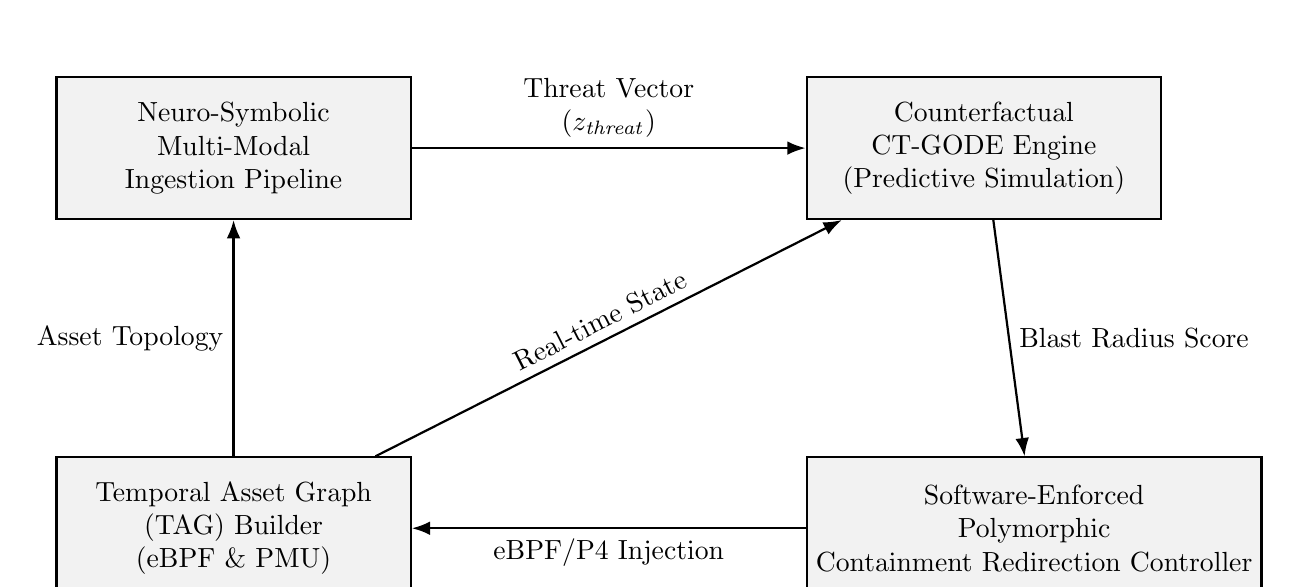
\begin{tikzpicture}[
  node distance=3cm and 5cm,
  box/.style={rectangle, draw, thick, minimum width=4.5cm, minimum height=1.8cm, align=center, fill=gray!10},
  arrow/.style={-Latex, thick}
]

% Nodes
\node (ingest) [box] {Neuro-Symbolic\\Multi-Modal\\Ingestion Pipeline};
\node (tag) [box, below=of ingest] {Temporal Asset Graph\\(TAG) Builder\\(eBPF \& PMU)};
\node (ctgode) [box, right=of ingest] {Counterfactual\\CT-GODE Engine\\(Predictive Simulation)};
\node (remedy) [box, right=of tag] {Software-Enforced\\Polymorphic\\Containment Redirection Controller};

% Arrows
\draw [arrow] (ingest) -- node[above, align=center] {Threat Vector\\($z_{\mathit{threat}}$)} (ctgode);
\draw [arrow] (tag) -- node[left] {Asset Topology} (ingest);
\draw [arrow] (tag) -- node[above, sloped] {Real-time State} (ctgode);
\draw [arrow] (ctgode) -- node[right] {Blast Radius Score} (remedy);
\draw [arrow] (remedy) -- node[below] {eBPF/P4 Injection} (tag);

\end{tikzpicture}
\caption{Schematic block diagram illustrating the overall system architecture.}
\label{fig:1}
\end{figure}

\begin{figure}[htbp]
\centering
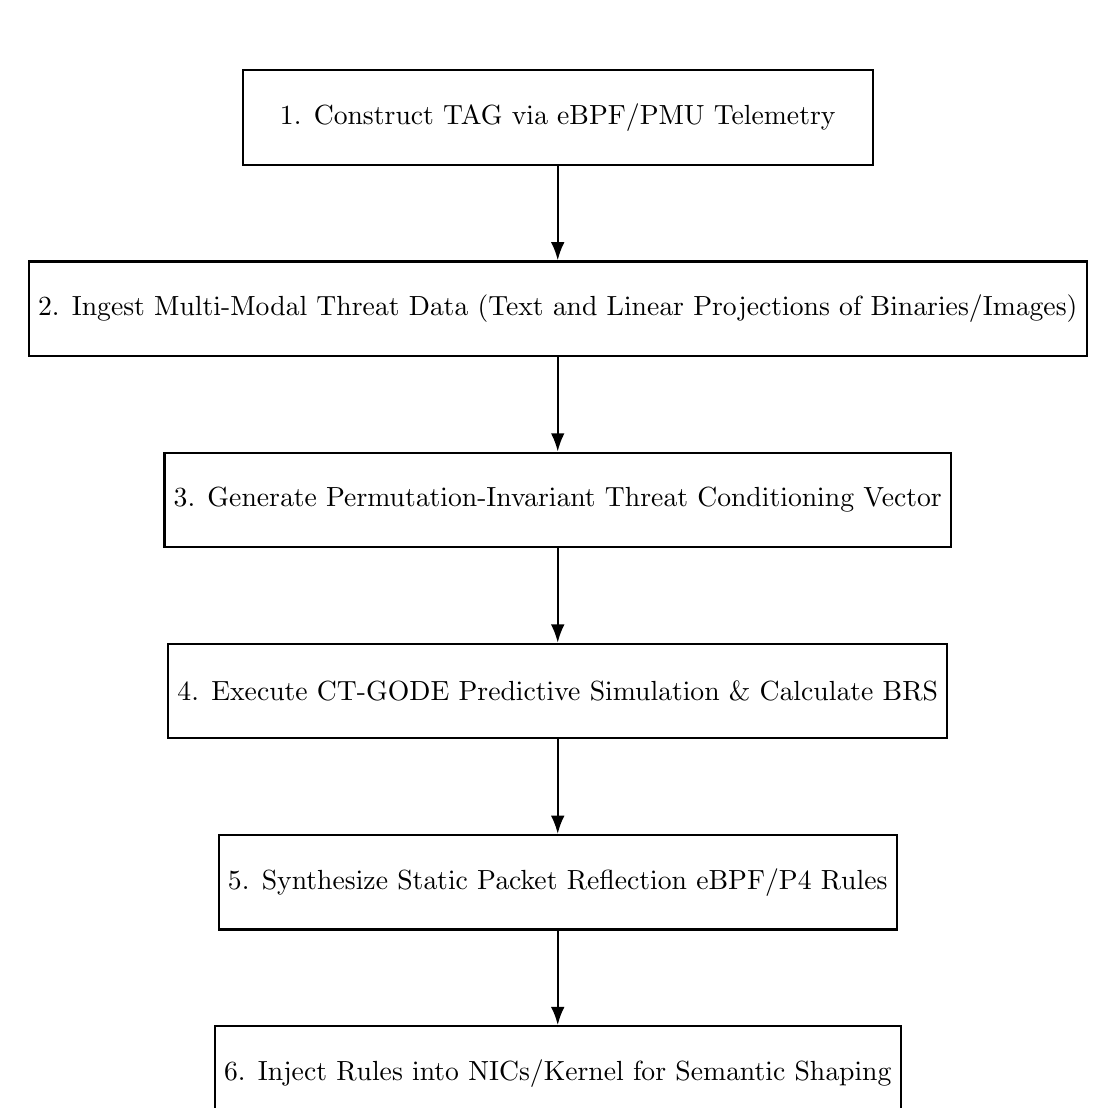
\begin{tikzpicture}[
  node distance=1.2cm,
  box/.style={rectangle, draw, thick, minimum width=8cm, minimum height=1.2cm, align=center},
  arrow/.style={-Latex, thick}
]

\node (step1) [box] {1. Construct TAG via eBPF/PMU Telemetry};
\node (step2) [box, below=of step1] {2. Ingest Multi-Modal Threat Data (Text and Linear Projections of Binaries/Images)};
\node (step3) [box, below=of step2] {3. Generate Permutation-Invariant Threat Conditioning Vector};
\node (step4) [box, below=of step3] {4. Execute CT-GODE Predictive Simulation \& Calculate BRS};
\node (step5) [box, below=of step4] {5. Synthesize Static Packet Reflection eBPF/P4 Rules};
\node (step6) [box, below=of step5] {6. Inject Rules into NICs/Kernel for Semantic Shaping};

\draw [arrow] (step1) -- (step2);
\draw [arrow] (step2) -- (step3);
\draw [arrow] (step3) -- (step4);
\draw [arrow] (step4) -- (step5);
\draw [arrow] (step5) -- (step6);

\end{tikzpicture}
\caption{Flowchart illustrating the preemptive threat containment redirection method.}
\label{fig:2}
\end{figure}

\begin{figure}[htbp]
\centering
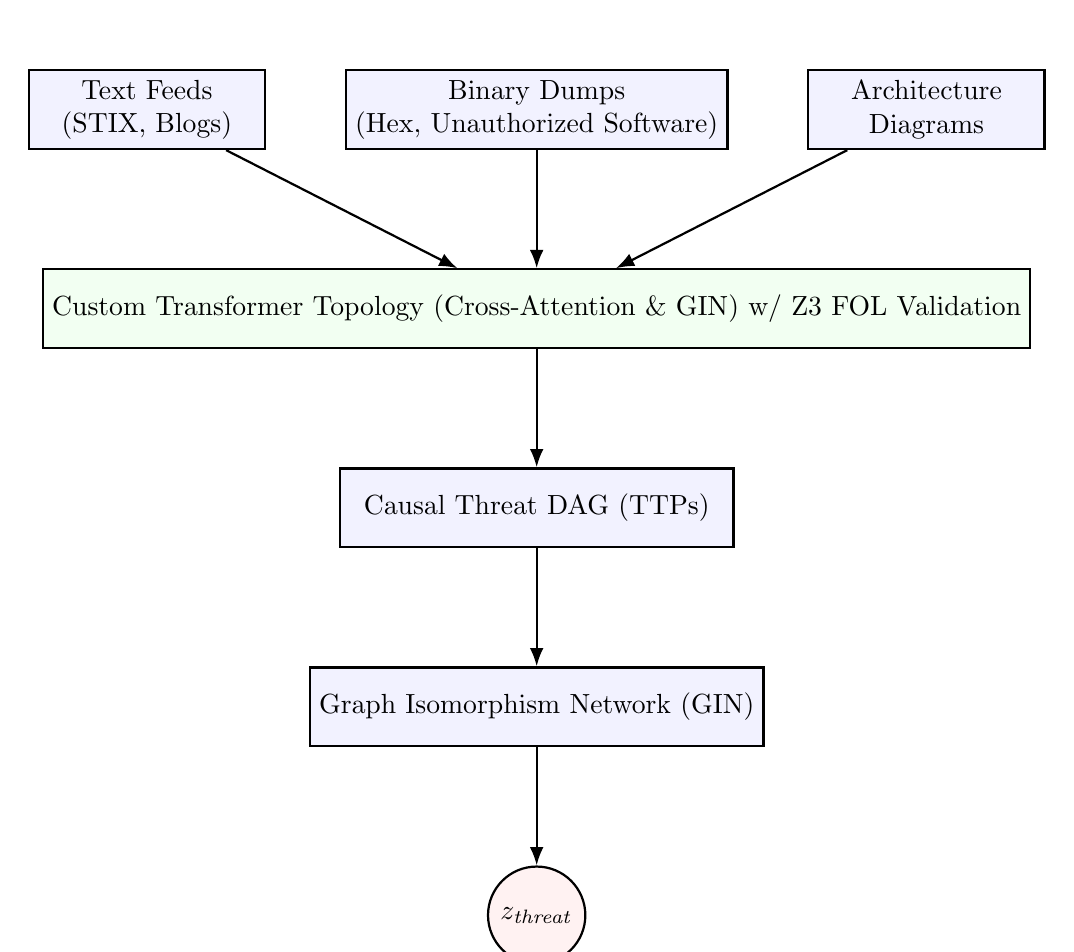
\begin{tikzpicture}[
  node distance=1.5cm and 1cm,
  box/.style={rectangle, draw, thick, minimum width=3cm, minimum height=1cm, align=center, fill=blue!5},
  circ/.style={circle, draw, thick, minimum size=1cm, align=center, fill=red!5},
  arrow/.style={-Latex, thick}
]

\node (text) [box] {Text Feeds\\(STIX, Blogs)};
\node (bin) [box, right=of text] {Binary Dumps\\(Hex, Unauthorized Software)};
\node (img) [box, right=of bin] {Architecture\\Diagrams};

\node (llm) [box, below=of bin, minimum width=10cm, fill=green!5] {Custom Transformer Topology (Cross-Attention \& GIN) w/ Z3 FOL Validation};

\node (dag) [box, below=of llm, minimum width=5cm] {Causal Threat DAG (TTPs)};
\node (gin) [box, below=of dag, minimum width=5cm] {Graph Isomorphism Network (GIN)};
\node (vector) [circ, below=of gin] {$z_{\mathit{threat}}$};

\draw [arrow] (text) -- (llm);
\draw [arrow] (bin) -- (llm);
\draw [arrow] (img) -- (llm);
\draw [arrow] (llm) -- (dag);
\draw [arrow] (dag) -- (gin);
\draw [arrow] (gin) -- (vector);

\end{tikzpicture}
\caption{Detailed block diagram of the Neuro-Symbolic Multi-Modal Ingestion Pipeline.}
\label{fig:3}
\end{figure}

\begin{figure}[htbp]
\centering
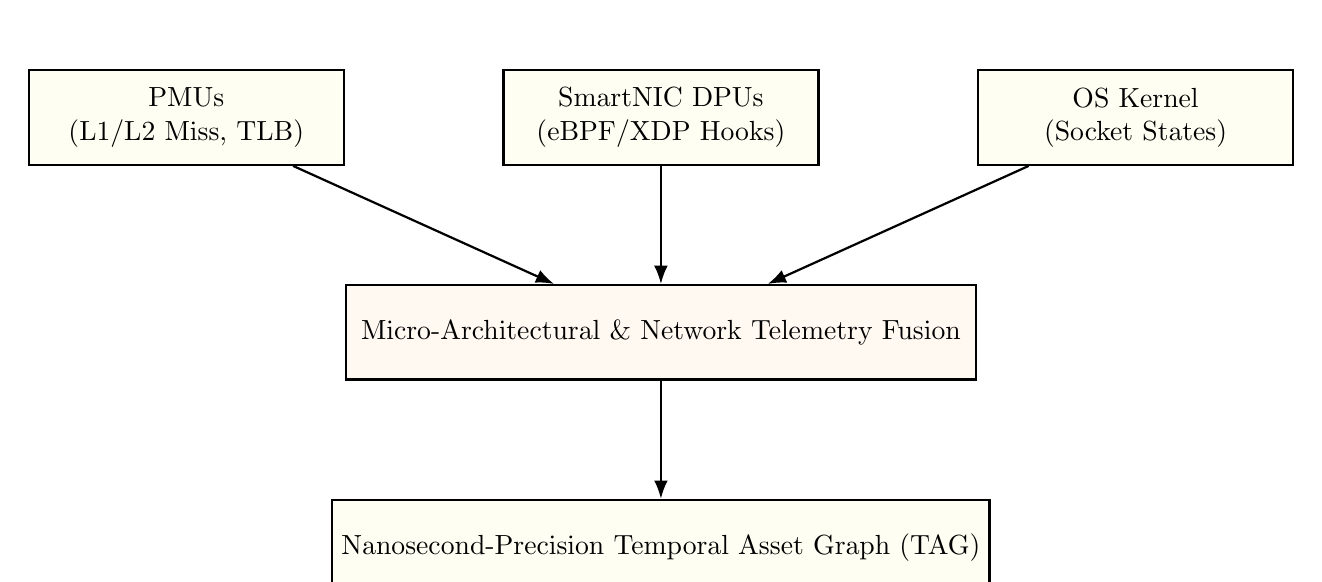
\begin{tikzpicture}[
  node distance=1.5cm and 2cm,
  box/.style={rectangle, draw, thick, minimum width=4cm, minimum height=1.2cm, align=center, fill=yellow!5},
  arrow/.style={-Latex, thick}
]

\node (cpu) [box] {PMUs\\(L1/L2 Miss, TLB)};
\node (nic) [box, right=of cpu] {SmartNIC DPUs\\(eBPF/XDP Hooks)};
\node (kernel) [box, right=of nic] {OS Kernel\\(Socket States)};

\node (fusion) [box, below=of nic, minimum width=8cm, fill=orange!5] {Micro-Architectural \& Network Telemetry Fusion};
\node (tag) [box, below=of fusion, minimum width=6cm] {Nanosecond-Precision Temporal Asset Graph (TAG)};

\draw [arrow] (cpu) -- (fusion);
\draw [arrow] (nic) -- (fusion);
\draw [arrow] (kernel) -- (fusion);
\draw [arrow] (fusion) -- (tag);

\end{tikzpicture}
\caption{Construction of the Temporal Asset Graph (TAG) via hardware and kernel telemetry.}
\label{fig:4}
\end{figure}

\begin{figure}[htbp]
\centering
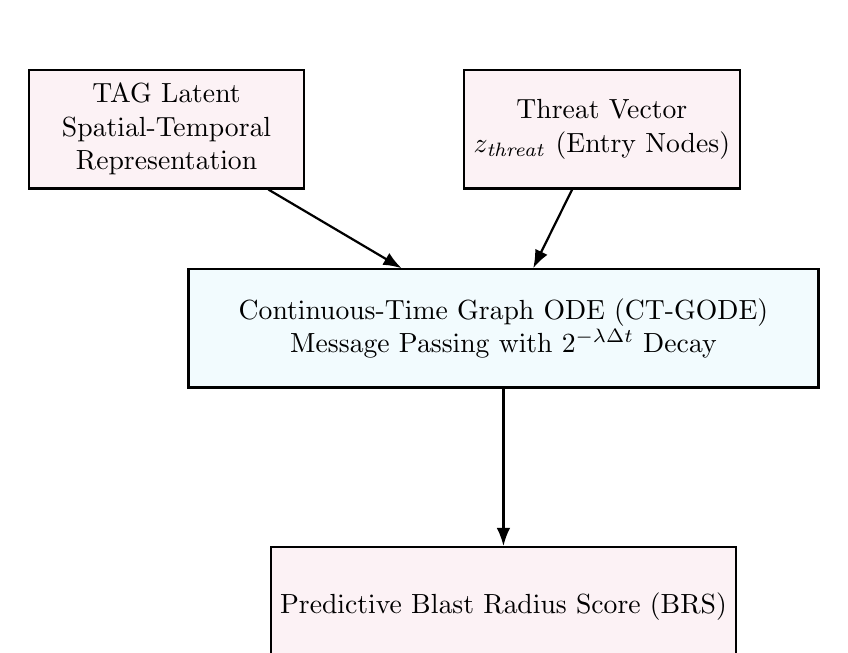
\begin{tikzpicture}[
  node distance=2cm and 2cm,
  box/.style={rectangle, draw, thick, minimum width=3.5cm, minimum height=1.5cm, align=center, fill=purple!5},
  arrow/.style={-Latex, thick}
]

\node (tag_input) [box] {TAG Latent\\Spatial-Temporal\\Representation};
\node (threat_input) [box, right=of tag_input] {Threat Vector\\$z_{\mathit{threat}}$ (Entry Nodes)};

\node (ctgode) [box, below right=1cm and -1.5cm of tag_input, minimum width=8cm, fill=cyan!5] {Continuous-Time Graph ODE (CT-GODE)\\Message Passing with $2^{-\lambda \Delta t}$ Decay};

\node (brs) [box, below=of ctgode] {Predictive Blast Radius Score (BRS)};

\draw [arrow] (tag_input) -- (ctgode);
\draw [arrow] (threat_input) -- (ctgode);
\draw [arrow] (ctgode) -- (brs);

\end{tikzpicture}
\caption{Functional diagram of the Counterfactual Continuous-Time Graph Neural Network (C-TGNN).}
\label{fig:5}
\end{figure}

\begin{figure}[htbp]
\centering
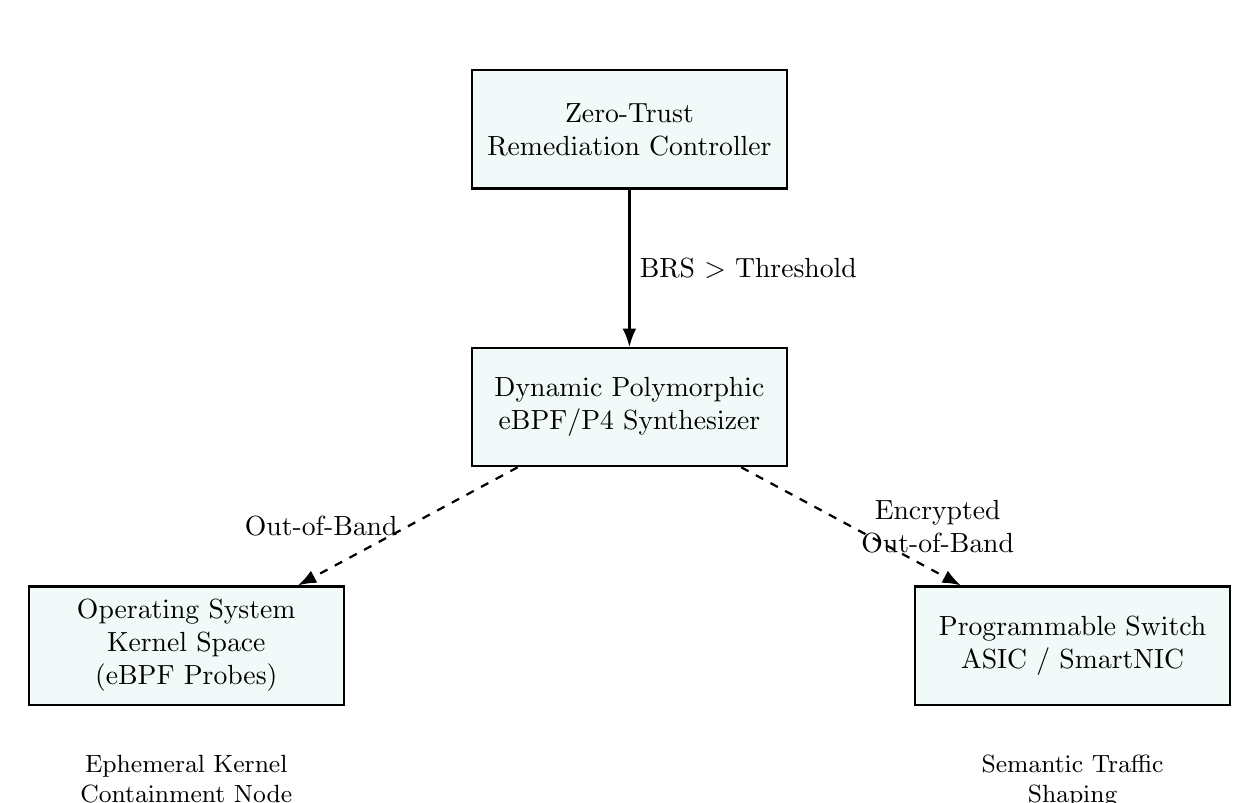
\begin{tikzpicture}[
  node distance=2cm and 2cm,
  box/.style={rectangle, draw, thick, minimum width=4cm, minimum height=1.5cm, align=center, fill=teal!5},
  arrow/.style={-Latex, thick, dashed}
]

\node (ctrl) [box] {Zero-Trust\\Remediation Controller};
\node (synth) [box, below=of ctrl] {Dynamic Polymorphic\\eBPF/P4 Synthesizer};

\node (tee) [box, below left=1.5cm and 1.6cm of synth] {Operating System\\Kernel Space\\(eBPF Probes)};
\node (asic) [box, below right=1.5cm and 1.6cm of synth] {Programmable Switch\\ASIC / SmartNIC};

\draw [-Latex, thick] (ctrl) -- node[right] {BRS $>$ Threshold} (synth);
\draw [arrow] (synth) -- node[left, align=center] {Out-of-Band} (tee);
\draw [arrow] (synth) -- node[right, align=center] {Encrypted\\Out-of-Band} (asic);

\node [below=0.5cm of tee, font=\small, align=center] {Ephemeral Kernel\\Containment Node};
\node [below=0.5cm of asic, font=\small, align=center] {Semantic Traffic\\Shaping};

\end{tikzpicture}
\caption{Static eBPF Packet Reflector Controller and out-of-band injection.}
\label{fig:6}
\end{figure}

\section{Detailed Description}
The present disclosure will now be described more fully hereinafter with reference to specific embodiments. The invention may, however, be embodied in many different forms and should not be construed as limited to the embodiments set forth herein. Furthermore, any specific mathematical dimensions, tensor sizes, or numerical configurations (e.g., embedding dimensions such as text\_dim=768) utilized in the system's implementation are expressly exemplary and non-limiting, and are provided solely to illustrate a reduction to practice without restricting the scope of the claims. 

\subsection{Cloud-Native SaaS Abstraction Layer and Swarm Intelligence}
In some embodiments, the system provides a Cloud-Native SaaS abstraction layer that aggregates telemetry from the eBPF probes into a centralized or distributed cloud environment. This tier establishes a Cloud-Native Swarm Intelligence network, allowing mid-market implementations to leverage the Counterfactual Threat Simulation Engine and predictive analytics without requiring out-of-band hardware components. The Cloud-Native SaaS tier functions as a base tier, which may optionally integrate with a \textbf{Software Implementation} tier for utilizing DPUs and SmartNICs to enforce full zero-trust hardware-enforced remediation.

\subsection{Threat Intelligence Ingestion via Neuro-Symbolic Multi-Modal Pipelines}
The system initiates by aggregating heterogeneous data streams, encompassing both structured feeds (e.g., STIX/TAXII) and highly unstructured sources. Crucially, the system utilizes a multi-modal approach, ingesting not only natural language text (e.g., dark web forums, cybersecurity advisories) but also alternative modalities such as compiled binary code snippets, hexadecimal memory dumps, and image-based architectural diagrams of observed threat infrastructure. In the event of a topological void where a specific data modality is unavailable, the pipeline mathematically maintains structural integrity by inserting a zero-padded tensor. 

In a preferred embodiment, the structured threat intelligence ingestion pipeline includes an automated fetching module configured to query and retrieve live Structured Threat Information Expression (STIX) threat datasets directly from the MITRE Cyber Threat Intelligence (CTI) repository. The retrieved threat intelligence is processed, parsed, and populated into a localized threat repository. To enable dynamic, real-time integration with downstream telemetry and orchestration layers, the system instantiates a production-ready FastAPI backend API. This backend exposes structured endpoints that serve the parsed threat vectors, dynamic telemetry analytics, and executive return-on-investment (ROI) data directly to the user dashboard and the TEE/eBPF controllers, establishing a low-latency feedback loop for zero-trust enforcement.

Unlike conventional language models susceptible to stochastic hallucination, the present invention employs a Neuro-Symbolic AI abstraction layer. This layer fuses a custom transformer topology (implemented as a 2-layer, 2-attention-head BERT transformer model, and incorporating Cross-Attention and a Graph Isomorphism Network) with deterministic First-Order Logic validation via Z3. To ensure bounded solver execution times, the First-Order Logic validation is applied strictly to specific security dimensions—namely, the first three dimensions representing complexity, severity, and impact—of the fused embedding. Unstructured threat intelligence is ingested into a Federated Learning pipeline secured via localized network policies. The custom transformer topology constructs a Causal Threat Directed Acyclic Graph (DAG), where nodes represent discrete Tactics, Techniques, and Procedures (TTPs) and directed edges represent temporal preconditions. This DAG is processed via a Graph Isomorphism Network (GIN) to generate a permutation-invariant Threat Conditioning Vector ($z_{\mathit{threat}}$), which encapsulates the topological and sequential nature of the attack, mapping semantic threat indicators into a Hyper-Dimensional Vector Space and absolutely guaranteeing the structural integrity of the generated Threat Embeddings.

\subsection{Dynamic Topology Generation via eBPF, XDP, and PMU Telemetry}
To achieve zero-overhead topological mapping, the system eschews host-CPU bound polling. Instead, it deploys polyglot extended Berkeley Packet Filter (eBPF) byte-code directly into the embedded ARM cores of DPUs and SmartNICs via eXpress Data Path (XDP) hooks. Furthermore, the telemetry engine dynamically fuses network socket states with deep micro-architectural telemetry harvested from CPU Performance Monitor Units (PMUs). 

To enable continuous telemetry simulation when physical hardware registers are offloaded or unavailable, PMU metrics (such as branch misses and TLB misses) are simulated directly inside the eBPF probe, specifically by taking kernel time modulo operations. By analyzing these simulated or physical metrics (including L1/L2 cache miss rates, branch prediction anomalies, and Translation Lookaside Buffer (TLB) thrashing) in conjunction with eBPF network telemetry, the system constructs a highly granular, nanosecond-precision Temporal Asset Graph (TAG). This enables the deterministic detection of pre-execution, memory-resident side-channel precursors (e.g., speculative execution variants) long before network communication occurs. The speed and volume at which the TAG is updated and the eBPF filters are compiled and injected (sub-millisecond intervals) vastly exceed human cognitive capacity, effectively preempting any capability for mental execution or manual processes.

\subsection{Continuous-Time Graph ODEs (CT-GODE) and Counterfactual Simulation}
Traditional discrete-time graph message passing fundamentally fails to capture the asynchronous, continuous nature of cyber-kinetic propagation. The core computational engine thus utilizes a Continuous-Time Dynamic Graph (CTDG) framework based on Neural Ordinary Differential Equations (NODEs) on Graphs, referred to herein as a Counterfactual Temporal Graph Neural Network (C-TGNN).

During periods absent of active threat intelligence, the system's custom transformer topology acts as a Generative Adversarial Network (GAN), synthesizing novel, counterfactual Threat Embeddings representing zero-day variations of known TTPs. The C-TGNN continuously projects these synthetic embeddings onto the evolving TAG to perform adversarial message passing. This continuous background simulation yields a Latent Structural Fragility Score for the topology, identifying topological vulnerabilities that exist independent of known exploits. 

When actual threat intelligence is ingested, the Threat Conditioning Vector ($z_{\mathit{threat}}$) is mapped to specific entry nodes. The mapping is achieved by correlating the Initial Access phase of the extracted TTPs (e.g., an exploited vulnerability in a specific library) with the software inventory and exposed network ports of nodes within the TAG. The system then executes Threat-Conditioned Continuous-Time Message Passing. For a given edge $e_{uv}(t)$ between nodes $u$ and $v$ at time $t$, the traversal probability weight $\alpha_{uv}(t)$ is computed via a cross-attention mechanism conditioned on the threat vector:
$$\alpha_{uv}(t) = \text{Softmax}(\text{LeakyReLU}(W_a [ h_u(t) \,\|\, h_v(t) \,\|\, e_{uv}(t) \,\|\, z_{\mathit{threat}} ]))$$
where $h_u(t)$ and $h_v(t)$ are the dynamic hidden states of the nodes updated via a memory module processing asynchronous eBPF events. 

In this process, the message vectors traversing the edges are subjected to a specific time-decay function. The probability of lateral movement is modified by a base-2 bitwise exponential time-decay factor $2^{-\lambda \Delta t}$, where $\lambda$ represents the temporal staleness of the threat intelligence. This ensures the resulting Blast Radius Score (BRS) accurately reflects a continuous, time-decaying predictive exposure metric. To achieve sub-millisecond scaling, the C-TGNN mathematical weights are computed via software simulation, enabling decentralized, swarm-based predictive consensus natively via inter-node network packets.

\subsection{Autonomous Static Packet Reflection and Software-Attested Remediation}
To ensure remediation persistence against kernel-level rootkits, the autonomous controller operates entirely out-of-band utilizing a Cryptographic Attestation protocol within a physical hardware Trusted Execution Environment (TEE) such as Intel SGX. During the cryptographic attestation lifecycle, the enclave compilation process executes compiler commands using host triggers. Upon the C-TGNN determining a critical BRS threshold, the controller eschews traditional binary blocking. Instead, the controller synthesizes and automatically updates statically pre-compiled eBPF maps for the packet reflector tailored to the specific predicted threat vector. 

These transient eBPF programs, and associated polymorphic P4-language routing logic, are pushed down via encrypted channels to programmable switch ASICs at the Top-of-Rack (ToR) and to the firmware of PCIe-attached DPUs at the Network Interface Controller (NIC) level. The executed eBPF program intercepts the predicted lateral movement attempts and fabricates protocol-compliant, synthetic responses, performing 'Semantic Traffic Shaping'. Specifically, the synthetic TCP sequence number ($\mathit{SEQ}_{\mathit{synth}}$) for the forged response is generated by XORing the source IP address, destination IP address, a decayed weight, and the current kernel time, according to the formula: $\mathit{SEQ}_{\mathit{synth}} = \mathit{IP}_{\mathit{src}} \oplus \mathit{IP}_{\mathit{dst}} \oplus W_{\mathit{decayed}} \oplus t_{\mathit{current}}$. This effectively transforms the vulnerable host into an ephemeral, kernel-level containment node, stalling the adversary without disrupting legitimate operations.

Furthermore, to maintain strict data privacy, the central processing module may be configured to execute the C-TGNN algorithm utilizing eBPF mapping. This allows the system to compute the spatial-temporal message passing securely. The invention fundamentally improves the functioning of the computer network by reducing the computational overhead of perimeter firewalls and localizing semantic shaping directly at the kernel and hardware layers.

\pagebreak
\section*{Claims}
\noindent \textbf{What is claimed is:}
\begin{enumerate}[label=\textbf{\arabic*.}, leftmargin=*]
    
    \item A computer-implemented method for pre-emptive, dynamic architectural reconfiguration and Hardware-Enforced threat containment redirection in a networked environment, the method comprising:
    \begin{enumerate}[label=(\alph*)]
        \item continuously constructing a nanosecond-precision Temporal Asset Graph (TAG) representing dynamic states of compute nodes and edges within a target environment via polyglot extended Berkeley Packet Filter (eBPF) probes;
        \item generating a permutation-invariant Threat Conditioning Vector by parsing multi-modal cybersecurity intelligence data utilizing a Neuro-Symbolic Artificial Intelligence pipeline comprising a custom transformer topology (incorporating Cross-Attention and a Graph Isomorphism Network) with deterministic First-Order Logic validation via Z3;
        \item determining a predicted lateral movement pathway through the target environment by executing a Continuous-Time Graph Ordinary Differential Equation (CT-GODE) algorithm that projects the Threat Conditioning Vector onto the TAG and performs spatial-temporal message passing natively orchestrated across nodes;
        \item automatically updating statically pre-compiled eBPF maps based strictly on the predicted lateral movement pathway determined by the CT-GODE algorithm; and
        \item pre-emptively isolating susceptible compute nodes by updating a statically pre-compiled map array within the static eBPF packet reflector directly into an out-of-band network controller and operating system kernel space of the susceptible compute nodes, wherein the eBPF program intercepts adversarial traffic and fabricates protocol-compliant synthetic responses at a network interface controller (NIC) level, thereby physically transforming the susceptible compute nodes into ephemeral kernel-level containment nodes and severing the predicted lateral movement pathway prior to active exploitation.
    \end{enumerate}

    \item The method of claim 1, wherein the extended Berkeley Packet Filter (eBPF) probes and Performance Monitor Units (PMUs) are offloaded to DPUs.

    \item The method of claim 1, wherein parsing the multi-modal cybersecurity intelligence data comprises ingesting not only natural language text, but also compiled binary code snippets, hexadecimal memory dumps, and image-based architectural diagrams, and fusing the multi-modal data utilizing cross-attention mechanisms.

    \item The method of claim 1, wherein the PMUs dynamically analyze L1 and L2 cache miss rates, branch prediction anomalies, and Translation Lookaside Buffer (TLB) thrashing to preemptively detect pre-execution, memory-resident side-channel precursors.

    \item The method of claim 1, further comprising executing a Counterfactual Threat Simulation Engine (CTSE) during periods absent of active threat intelligence, wherein the CTSE utilizes a Permutation-Invariant Counterfactual Engine to synthesize and inject counterfactual zero-day threat embeddings into the CT-GODE algorithm to calculate a Latent Structural Fragility Score for the target environment.

    \item The method of claim 1, wherein the Threat Conditioning Vector is mapped to specific entry nodes on the TAG by correlating an Initial Access phase of an extracted threat payload with a software inventory and exposed network ports of the compute nodes.

    \item The method of claim 1, wherein the decentralized spatial-temporal message passing computes a traversal probability weight for a given edge that is continuously modified by an exponential time-decay factor $2^{-\lambda \Delta t}$ computed via floating-point or bitwise operations, wherein $\lambda$ represents a temporal staleness of the cybersecurity intelligence data.

    \item A system for pre-emptive cybersecurity defense and automated architectural reconfiguration, the system comprising:
    \begin{enumerate}[label=(\alph*)]
        \item at least one memory storing computer-executable instructions; and
        \item at least one hardware processor coupled to the at least one memory, wherein the at least one hardware processor is configured to execute the instructions to:
        \begin{enumerate}[label=\roman*.]
            \item intercept, via Performance Monitor Units (PMUs) and extended Berkeley Packet Filter (eBPF) kernel probes, deep micro-architectural telemetry and dynamic inter-process communications across a networked enterprise environment to construct a real-time Temporal Asset Graph (TAG);
            \item process multi-modal threat intelligence streams, including text, compiled binary code snippets, and architectural diagrams, utilizing a Neuro-Symbolic Artificial Intelligence layer to output a Causal Threat Directed Acyclic Graph (DAG);
            \item continuously synthesize permutation-invariant counterfactual zero-day threats by projecting counterfactual embeddings onto a latent spatial-temporal representation of the TAG;
            \item determine a continuous, time-decaying predictive exposure metric for distinct sub-components of the networked enterprise environment by applying a CT-GODE algorithm over the latent spatial-temporal representation; and
            \item synthesize and dynamically inject Static Packet Reflection rules and routing logic directly into host-level kernel space via eBPF, or via encrypted out-of-band channels to programmable switch Application-Specific Integrated Circuits (ASICs).
        \end{enumerate}
    \end{enumerate}

    \item The system of claim 8, wherein the Static Packet Reflection rules configure the specific host machines to perform Semantic Traffic Shaping by intercepting predicted lateral movement attempts and fabricating protocol-compliant, synthetic responses.

    \item The system of claim 8, wherein the predictive exposure metric is calculated at sub-millisecond intervals utilizing mathematical weights distributed directly to the eBPF kernel probes, thereby bypassing centralized correlation engines and enabling pre-emptive hardware-enforced reconfiguration of network architecture.

    \item The system of claim 8, wherein the Cryptographic Attestation protocol is configured to execute within a physical hardware Trusted Execution Environment (TEE) such as Intel SGX, wherein the synthesis and injection of the Static Packet Reflection rules and routing logic is strictly conditioned upon cryptographic validation of a Hardware-Enforced license topology corresponding to the specific host machines and switch ASICs.

    \item The system of claim 8, wherein the Semantic Traffic Shaping synthesizes TCP SYN-ACK responses using a formula $\mathit{SEQ}_{\mathit{synth}} = \mathit{IP}_{\mathit{src}} \oplus \mathit{IP}_{\mathit{dst}} \oplus W_{\mathit{decayed}} \oplus t_{\mathit{current}}$.

\end{enumerate}

\end{document}